\chapter{Classically accelerating solenoidal wave packets in two dimensions}
\label{ch:accelerating}


In 1979, Balazs and Berry reported the discovery of
shape-preserving wave packets for quantum mechanical particles
that translate with uniform
acceleration in one dimension \cite{balazs79}.
Taking the form of Airy functions, these wave packets
appear to violate Ehrenfest's theorem because
they accelerate in the absence of any applied force.
This conundrum is resolved by recognizing that an
Airy wave packet is not
square-integrable and thus is best interpreted as an 
ensemble of non-accelerating single-particle plane-wave states \cite{balazs79,ballentine94}.
Optical analogs to Airy wave packets
have been realized in holographically-patterned laser beams,
the temporal evolution of the quantum state being modeled through
the spatial evolution of the light's intensity profile
\cite{siviloglou07,siviloglou07a,kaminer12}.
In this case, the beam's intensity profile translates
along a parabolic path as it propagates, without
otherwise distorting.
The analogy between the spatial structure of a propagating
light beam and the temporal evolution of a quantum
mechanical wave packet reflects the homology of 
the paraxial wave equation with Schr\"odinger's equation.

Here, we introduce an alternative class of shape-preserving wave
packets in two dimensions \cite{Mondal_accelerating} 
that describe a particle undergoing
uniform circular motion
in the force-free region of a circular box.
Although the confined wave packet's time evolution is consistent with
Ehrenfest's theorem, the equivalent truncated wave packet in free
space appears to accelerate in the absence of a central force.
Rotating states also have the surprising property that
the classical angular momentum they carry
differs from their quantum mechanical angular momentum,
and indeed can have the opposite sign.
We illustrate these properties through experimental realizations
of analogous propagation-invariant laser modes projected
with intermediate-plane
holography \cite{mondal18}.

The wave function, $\Psi(\vec{r})$, of a nonrelativistic particle of mass $m$
moving in a two-dimensional circular box of radius $R$ can be
expressed in polar coordinates, $\vec{r} = (r, \phi)$,
in terms of eigenfunctions of
the force-free 
time-independent Schr\"odinger equation,
\begin{subequations}
  \label{eq:se}
\begin{equation}
  \label{eq:schrodinger}
  - \frac{\hbar^2}{2m} \, \nabla^2
  \Psi(\vec{r})
  =
  E \, \Psi(\vec{r}),
\end{equation}
with polar Laplacian
\begin{equation}
  \label{eq:laplacian}
  \nabla^2 =
  \frac{\partial^2}{\partial r^2} + \frac{1}{r} \frac{\partial}{\partial r}
  + \frac{1}{r^2} \frac{\partial^2}{\partial \phi^2},
\end{equation}
subject to the boundary condition 
\begin{equation}
  \label{eq:boundarycondition}
  \Psi(R, \phi) = 0 .
\end{equation}
\end{subequations}
Equation~\eqref{eq:se} is satisfied by the Bessel wave functions,
$\ket{n, \nu}$, whose spatial representation is
\begin{subequations}
      \label{eq:eigenstates}
\begin{align}
  \label{eq:besselstates}
  \Psi_{n,\nu}(\vec{r})
  & =
    \braket{\vec{r} | n,\nu} \\
  & =
    A_{n,\nu} \, J_n\left(j_{n,\nu} \frac{r}{R}\right) \, e^{i n \phi} ,
\end{align}
where $J_n(x)$ is a Bessel function of the first kind of order $n$,
and where $j_{n,\nu}$ is its $\nu$-th zero.
The prefactor
\begin{equation}
  \label{eq:normalization}
  A_{n,\nu} = \left[\pi^{1/2} R \, J_{n+1}(j_{n,\nu})\right]^{-1}
\end{equation}
\end{subequations}
ensures that the corresponding probability density
\begin{equation}
  \label{eq:probabilitydensity}
  \rho_{n,\nu}(\vec{r})
  =
  \abs{\Psi_{n,\nu}(\vec{r})}^2,
\end{equation}
is properly normalized.
The Bessel states then are orthonormal:
\begin{equation}
  \label{eq:orthonormality}
  \braket{n', \nu' | n, \nu}
  =
  \delta_{n,n'} \delta_{\nu, \nu'}.
\end{equation}
Their eigenenergies,
\begin{equation}
  \label{eq:eigenenergy}
  E_{n,\nu} =
  \frac{\hbar^2 j_{n,\nu}^2}{2 m R^2},
\end{equation}
depend on both the azimuthal quantum number, $n$,
and the radial quantum number, $\nu$.
The associated frequency, $\omega_{n, \nu} = E_{n,\nu}/\hbar$,
establishes the eigenstates' time evolution,
\begin{equation}
  \label{eq:timedependent}
  \Psi_{n,\nu}(\vec{r},t) =
  \braket{\vec{r} | n, \nu} \, e^{-i \omega_{n,\nu} t}.
\end{equation}

The states described by Eqs.~\eqref{eq:eigenstates} and \eqref{eq:timedependent}
are analogous to optical Bessel beams \cite{durnin87,durnin87a}, 
with the time in
Eq.~\eqref{eq:timedependent}
serving as an analog to the light wave's axial coordinate.
Like their optical counterparts, Bessel wavefunctions
carry angular momentum with expectation value
\begin{equation}
  \label{eq:angularmomentum}
  \braket{L_z}
  =
  -i \hbar \,
  \int \Psi_{n,\nu}^\ast(\vec{r}) \frac{\partial}{\partial \phi}
  \Psi_{n,\nu}(\vec{r}) \, d^2r
  =
  n \hbar
\end{equation}
that depends on $n$, but not on $\nu$.
For optical Bessel beams, this orbital angular momentum is a classical
property of the electromagnetic field \cite{allen92,allen99} that
also is a quantum mechanical property of the individual photons
\cite{leach02}.
For the particle in a circular box, it is strictly a quantum mechanical
property.
The particle's probability density, $\rho_{n,\nu}(\vec{r})$,
is independent of time, which means that the particle
is stationary in the classical sense and therefore
carries no classical angular momentum.
Similar discrepancies between the classical and quantum mechanical
angular momentum have been noted for Landau states
in free electron beams \cite{schattschneider14}.

\begin{figure}[!t]
  \centering
  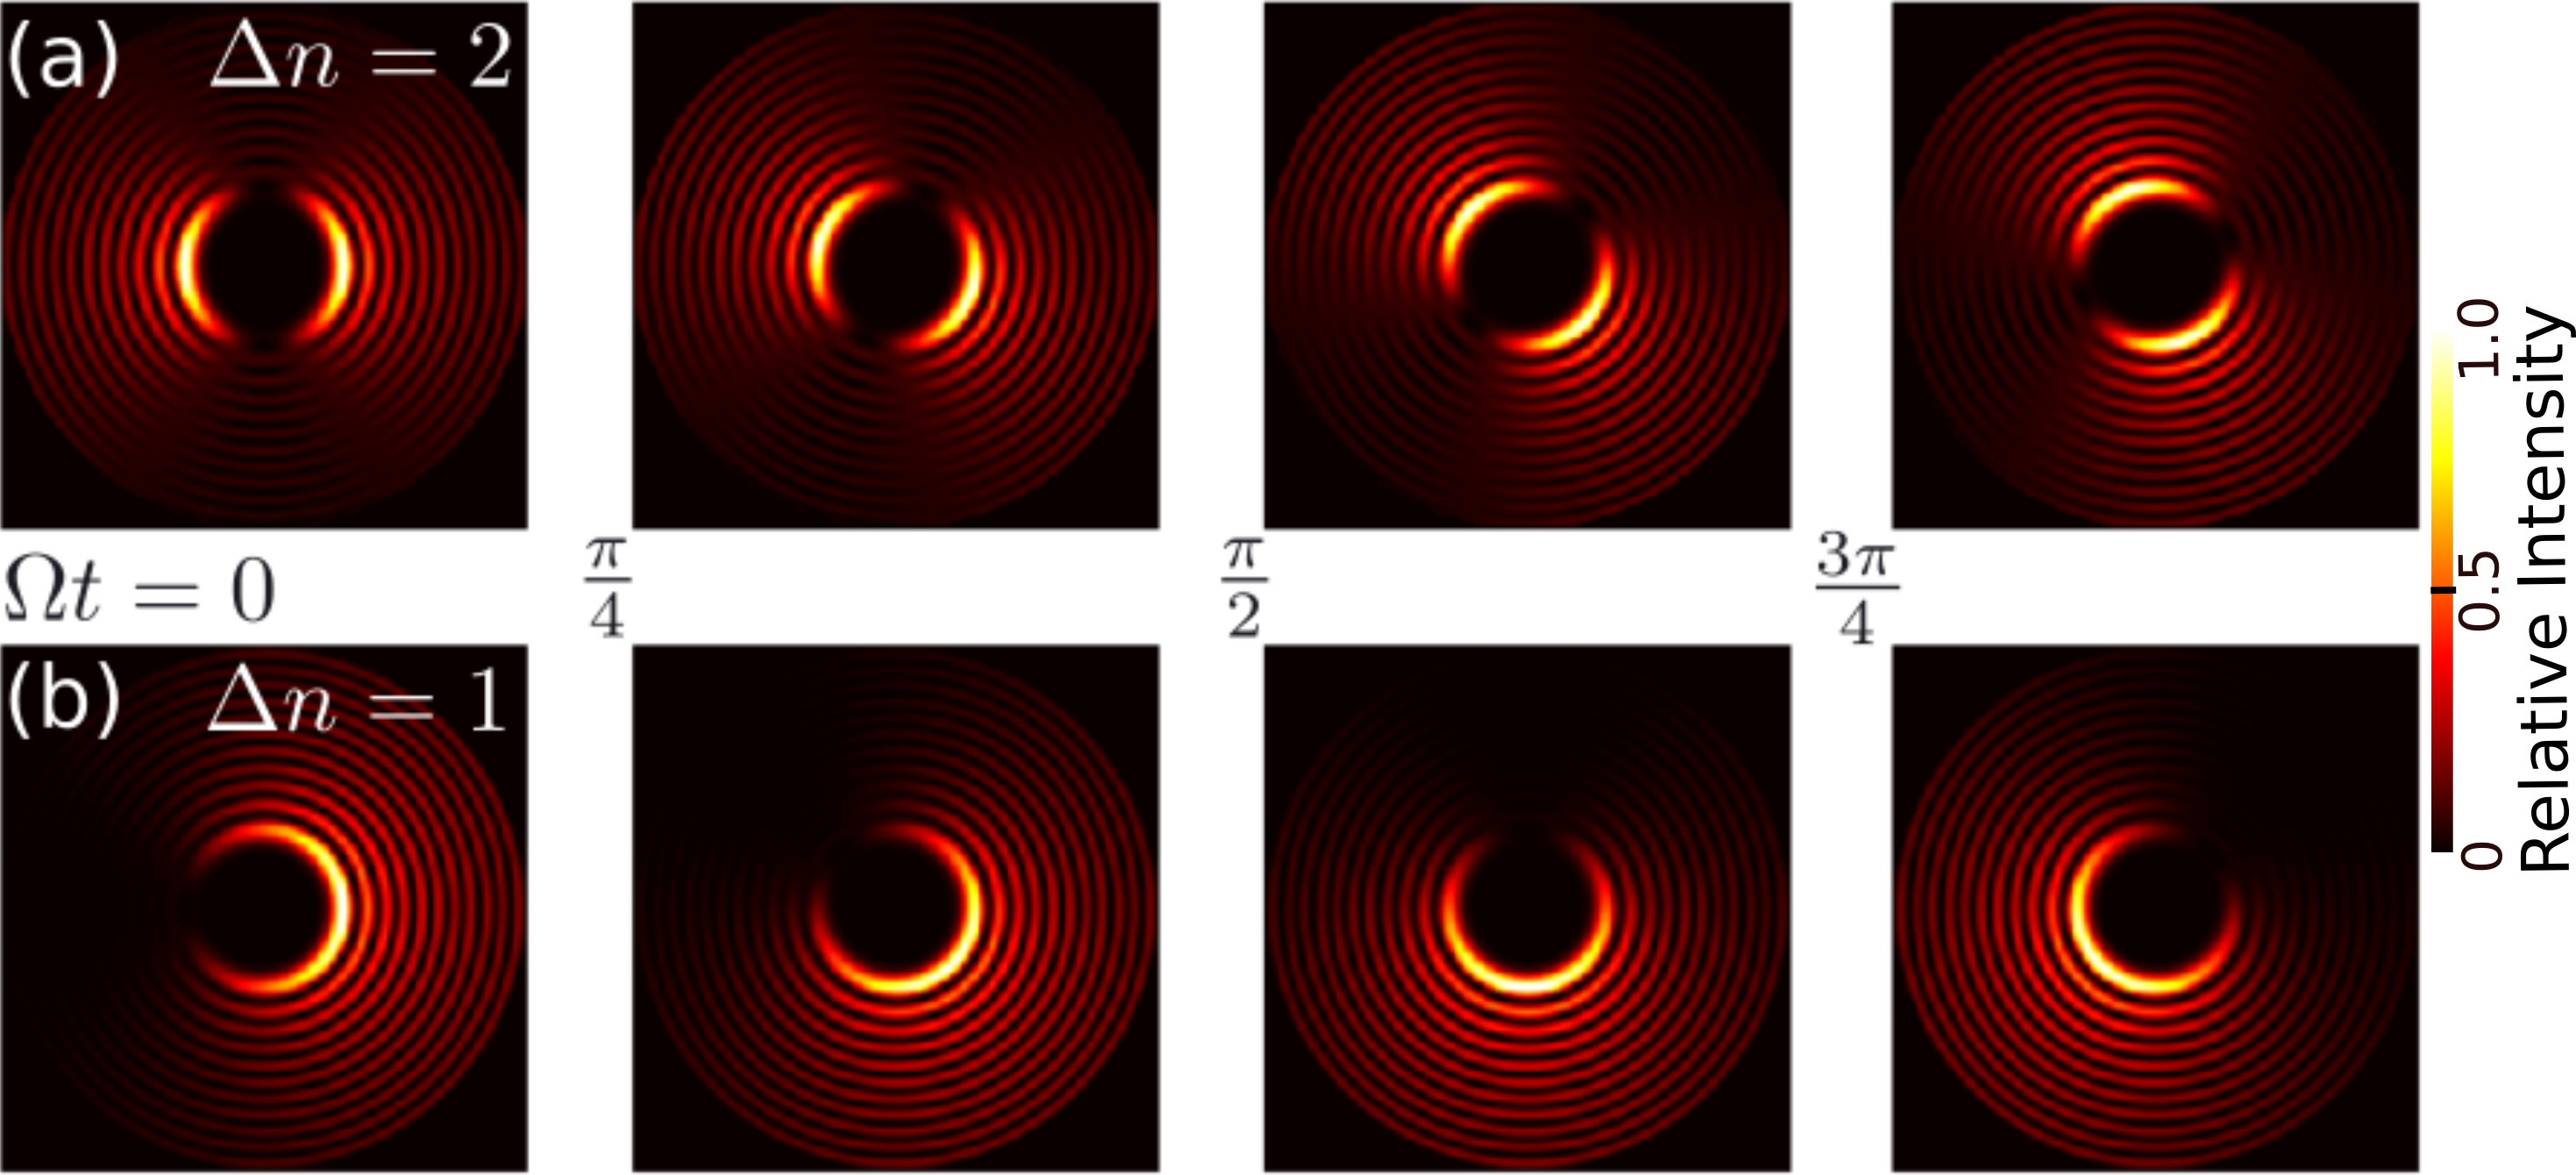
\includegraphics[width=\columnwidth]{rotation03}
  \caption{Rotation of solenoidal states with $n = 6$, $\nu = 15$,
    and $\nu' = \nu - 1$.  (a) Non-accelerating wave packet with
    $\Delta n = n' - n = 2$.
    (b) Accelerating state with $\Delta n = 1$.}
  \label{fig:solenoidalwave}
\end{figure}

Although individual Bessel eigenmodes are time-invariant,
some of their superpositions have probability densities that
rotate at a uniform rate without otherwise
distorting \cite{vasilyeu09,lee10,schulze15}.
Some of these rotating wave packets
constitute accelerating states in the sense that the
expectation value of the particle's position traces out an
accelerating trajectory.
These are not simply related to two-dimensional
Airy states or to related Matthieu and Weber states
\cite{zhang12nonparaxial} or to their generalizations
\cite{bandres13,chremmos13,zhao15shaping}, and thus constitute a distinct class
of accelerating states in two dimensions.

Minimal examples of rotating wave packets
can be constructed by superposing two Bessel states:
\begin{equation}
  \label{eq:solenoid}
  \Psi(\vec{r}, t)
  =
  \frac{1}{\sqrt{2}} \, \left[
    \Psi_{n,\nu}(\vec{r}, t) +
    \Psi_{n', \nu'}(\vec{r}, t)
  \right].
\end{equation}
For clarity, we arrange indices so that $\Delta n = n' - n > 0$.
This superposition's probability density
\begin{multline}
  \rho(\vec{r}, t)
  =
  \frac{1}{2} \, 
  \left[ \rho_{n,\nu}(\vec{r}) + \rho_{n',\nu'}(\vec{r}) \right] + \\
  \left[ \rho_{n,\nu}(\vec{r}) \rho_{n',\nu'}(\vec{r}) \right]^{1/2} \,
    \cos\left( \Delta n[ \phi - \Omega t] \right),
\end{multline}
rotates around the origin with an angular frequency
\begin{equation}
  \label{eq:frequency}
  \Omega = \frac{\hbar}{2m R^2} \,
  \frac{j_{n',\nu'}^2 - j_{n,\nu}^2}{\Delta n}.
\end{equation}
Aside from this rotation, the state neither broadens nor
otherwise distorts.
The resulting periodic recurrence differs from the
breathing modes identified in generalized Airy states
\cite{kaminer12}.
Instead, it closely resembles the discrete
propagation invariance of rotating optical modes \cite{tervo01},
particularly solenoidal beams \cite{lee10}.
For this reason, we refer to the rotating
wave functions described by Eq.~\eqref{eq:solenoid} as
solenoidal states.
Figure~\ref{fig:solenoidalwave} shows the time evolution of
two illustrative examples.

Most solenoidal wave packets are not accelerating states in the sense
identified by Balazs and Berry.
Those with $\Delta n > 1$, such as the example
in Fig.~\ref{fig:solenoidalwave}(a), are symmetric about the origin;
the expectation value of the particle's position coincides with
the center of the box.
Classically, therefore, such states resemble their constituent Bessel states
in that the particle remains motionless at the origin even as its
probability density rotates.

Solenoidal states with $\Delta n = 1$ are asymmetric,
as can be seen in Fig.~\ref{fig:solenoidalwave}(b).
The expectation value for the particle's position,
\begin{equation}
  \label{eq:position}
  \braket{\vec{r}(t)}
  =
  \alpha R \,
  \left[\cos(\Omega t) \, \hat{x} + \sin(\Omega t) \,
    \hat{y}\right], 
\end{equation}
undergoes uniform circulation motion at angular frequency
$\Omega$ and radius $\braket{r} = \alpha R$,
where
\begin{subequations}
  \label{eq:radius}
\begin{align}
  \alpha
  & =
  \frac {
    \int_0^1 J_{n+1}(j_{n+1,\nu'} x) \, J_n(j_{n, \nu} x) \, x^2 \, dx
  }{
    J_{n+2}(j_{n+1,\nu'}) \, J_{n+1}(j_{n,\nu})} \\
  & =
   \frac{2 j_{n+1,\nu'} j_{n,\nu}}{(j_{n+1,\nu'}^2 - j_{n,\nu}^2)^2}.
\end{align}
\end{subequations}
This seems remarkable because
no force acts on the particle within the box.
Such force-free acceleration appears
to violate Ehrenfest's theorem, which relates the expectation value of the
particle's acceleration to the expectation value of the force acting
on the particle,
\begin{equation}
  \label{eq:ehrenfest}
  \frac{d^2 \braket{\vec{r}(t)}}{dt^2}
  = \frac{1}{m} \braket{\vec{F}(\vec{r}(t))}.
\end{equation}
In the present case, $\vec{F}(\braket{\vec{r}(t)}) = 0$ in the force-free
region within the box, but
\begin{equation}
  \label{eq:violation}
  \frac{d^2 \braket{\vec{r}(t)}}{dt^2}
  =
  - \alpha R \, \Omega^2 \hat{r}.
\end{equation}
The apparent discrepancy can be explained because
$\vec{F}(\braket{\vec{r}(t)}) \neq \braket{\vec{F}(\vec{r}(t))}$.

\begin{figure*}[!t]
  \centering
  \includegraphics[width=0.95\textwidth]{light05}
  \caption{Optical realization of accelerating solenoidal states.
    Volumetric reconstructions of asymmetric solenoidal waves
    described by Eq.~\eqref{eq:solenoid} with $\Delta n = 1$.
    (a) Positive helicity: $n = 20$, $\nu = 15$, $\nu' = 14$.
    (b) Negative helicity: $\nu = 14$, $\nu' = 15$.
    (c) Four-mode ($n = 10$, 11, 12, 13) superposition yielding improved in-plane localization.}
  \label{fig:light}
\end{figure*}

The integrability of the solenoidal wave packets comes at
the cost of applying the boundary condition from Eq.~\eqref{eq:boundarycondition}
at $r = R$.
The confined particle exerts a pressure on the wall,
\begin{subequations}
  \label{eq:force}
  \begin{align}
    \label{eq:pressureprinciple}
    P
    & =
      - \frac{1}{2 \pi R} \frac{d E}{d R} \\
    & =
      \frac{\hbar^2}{4 \pi m R^4}
      \left(
      j_{n+1,\nu'}^2 + j_{n,\nu}^2
      \right).
      \label{eq:pressureactual}
  \end{align}
\end{subequations}
By Newton's third law, the wall exerts a complementary
force on the wave packet that is directed radially inward.
When averaged over angles, the net force acting on the
particle located at $\braket{\vec{r}}$ is
\begin{subequations}
  \label{eq:forceactual}
\begin{equation}
  \braket{\vec{F}(\vec{r})}
  = 
  - \beta R \, P \, \hat{r} ,
\end{equation}
where
\begin{align}
  \beta
  & =
    \lim_{\epsilon \to 0}
    \frac{\left.
    \int_0^{2\pi} \rho(\vec{r},t) \cos(\phi - \Omega t) \, d\phi
    \right\vert_{r = R - \epsilon}}
    {\left.
    \int_0^{2\pi} \rho(\vec{r},t) \, d\phi
    \right\vert_{r = R - \epsilon}} \\
  & =
    \frac{2 j_{n+1,\nu'}j_{n,\nu}}{
    j_{n+1,\nu'}^2 + j_{n,\nu}^2} .
\end{align}
\end{subequations}
Comparison with Eq.~\eqref{eq:violation} confirms
that Ehrenfest's theorem is satisfied: the force
responsible for the particle's classical circular
motion is exerted by the wave function's interaction
with the bounding wall.

In principle, accelerating solenoidal states can be prepared
as superpositions of Bessel beams without confining boundary conditions.
Such unconfined states rotate without a central force, and
so appear to violate Ehrenfest's theorem.
Because Bessel states
are not square-integrable, however, they are best
interpreted as superpositions of plane-wave states
\cite{balazs79}.
The rotation of solenoidal wave packets then 
represents the ensemble-averaged behavior of
multiple particles' non-accelerating trajectories.

The possibility of Ehrenfest violations arises again
for normalizable approximations to unconfined
solenoidal wave packets that are prepared by truncating
$\Psi(\vec{r},t)$ at $r = R$.
These truncated wave packets still appear to rotate,
and they evolve under truly force-free conditions.
To illustrate this phenomenon, Fig.~\ref{fig:light}
presents optical analogs of truncated solenoidal states.
We prepare these solenoidal beams of light
by using intermediate-plane holograms \cite{mondal18}
to convert the linearly polarized
Gaussian TEM$_{00}$ beam from
a solid state laser (Coherent Verdi 5W) into a superposition
of helical Bessel modes of the form described by
Eq.~\eqref{eq:solenoid}.
The mode-converting holograms are imprinted
on the beam with a phase-only liquid crystal 
spatial light modulator (Hamamatsu X10468-16).

Figure~\ref{fig:light}(a) and Fig.~\ref{fig:light}(b)
show volumetric reconstructions of two
solenoidal laser beams with $\Delta n = 1$.
The data for these reconstructions
were obtained by translating a video camera 
(NEC TI-324AII) along the optical axis and
combining the resulting stack of images.
Each reconstruction shows three complete cycles of shape-preserving
propagation.
The solenoid in Fig.~\ref{fig:light}(a) has a right-handed twist
while that in Fig.~\ref{fig:light}(b) is left-handed.
Each volumetric reconstruction is paired with three
transverse slices from the planes labeled
(i), (ii) and (iii) in the renderings.
These slices show three stages in the
intensity distributions' rotation about the optical axis at
\SI{120}{\degree} intervals.
Additional planes in the renderings
correspond to each of the three complete rotations
captured over the
course of \SI{1}{\meter} of propagation.  The full non-diffracting
range of these beams extends beyond \SI{2}{\meter}.

The two-state superpositions discussed so far are not
the only accelerating wave packets.
Figure~\ref{fig:light}(c) shows a four-state superposition
designed to optimally localize the wave packet as it spirals
around the origin.
In this case, there can be no doubt that the point of
maximum intensity rotates about the 
optical axis, and therefore that
the most probable particle position,
$\vec{r}^\ast(t)$, undergoes uniform
circular motion under force-free conditions.

Figure~\ref{fig:translation}(a)
shows a representative simulation of
$\vec{r}^\ast(t)$ superimposed on a snapshot
of the initial distribution, $\rho(\vec{r},0)$.
Figure~\ref{fig:translation}(b) shows the corresponding
experimental measurement of $\vec{r}^\ast(z)$.
The angular position of the peak, $\theta^\ast(t)$,
advances uniformly, as can be seen in Fig.~\ref{fig:translation}(c).
For clarity, we have scaled the simulation time to best
superimpose the temporal evolution of the simulation
data on the spatial evolution of the experimental data, $\theta^\ast(z)$.

This apparent contradiction of the Ehrenfest theorem
is resolved by tracking the mean particle position,
$\braket{\vec{r}(t)}$, which also is plotted
in Fig.~\ref{fig:translation}.
Results for $\braket{x(t)}$ and $\braket{x(z)}$ are plotted in
Fig.~\ref{fig:translation}(d), with the simulation
time again scaled as in Fig.~\ref{fig:translation}(c).
In both simulation and experiment, the
classical trajectory of the unconfined
rotating wave packet actually \emph{translates}
steadily away from the beam's axis with an
impact parameter, $b$ set by the average position
at $t = 0$.
This motion arises because the truncated
wave packet diffracts beyond $r = R$ by precisely
the amount needed to conserve momentum
under force-free conditions.
The nature of the state's time 
evolution is masked because diffraction has
little apparent influence on the wave packet's
structure at early times, particularly near
the center of the system.
Remarkably, this means that the 
finite-aperture solenoidal laser modes
presented in Fig.~\ref{fig:light} are not
accelerating states in the sense introduced
by Balasz and Berry, despite their
apparent rotation.

\begin{figure}
  \centering
  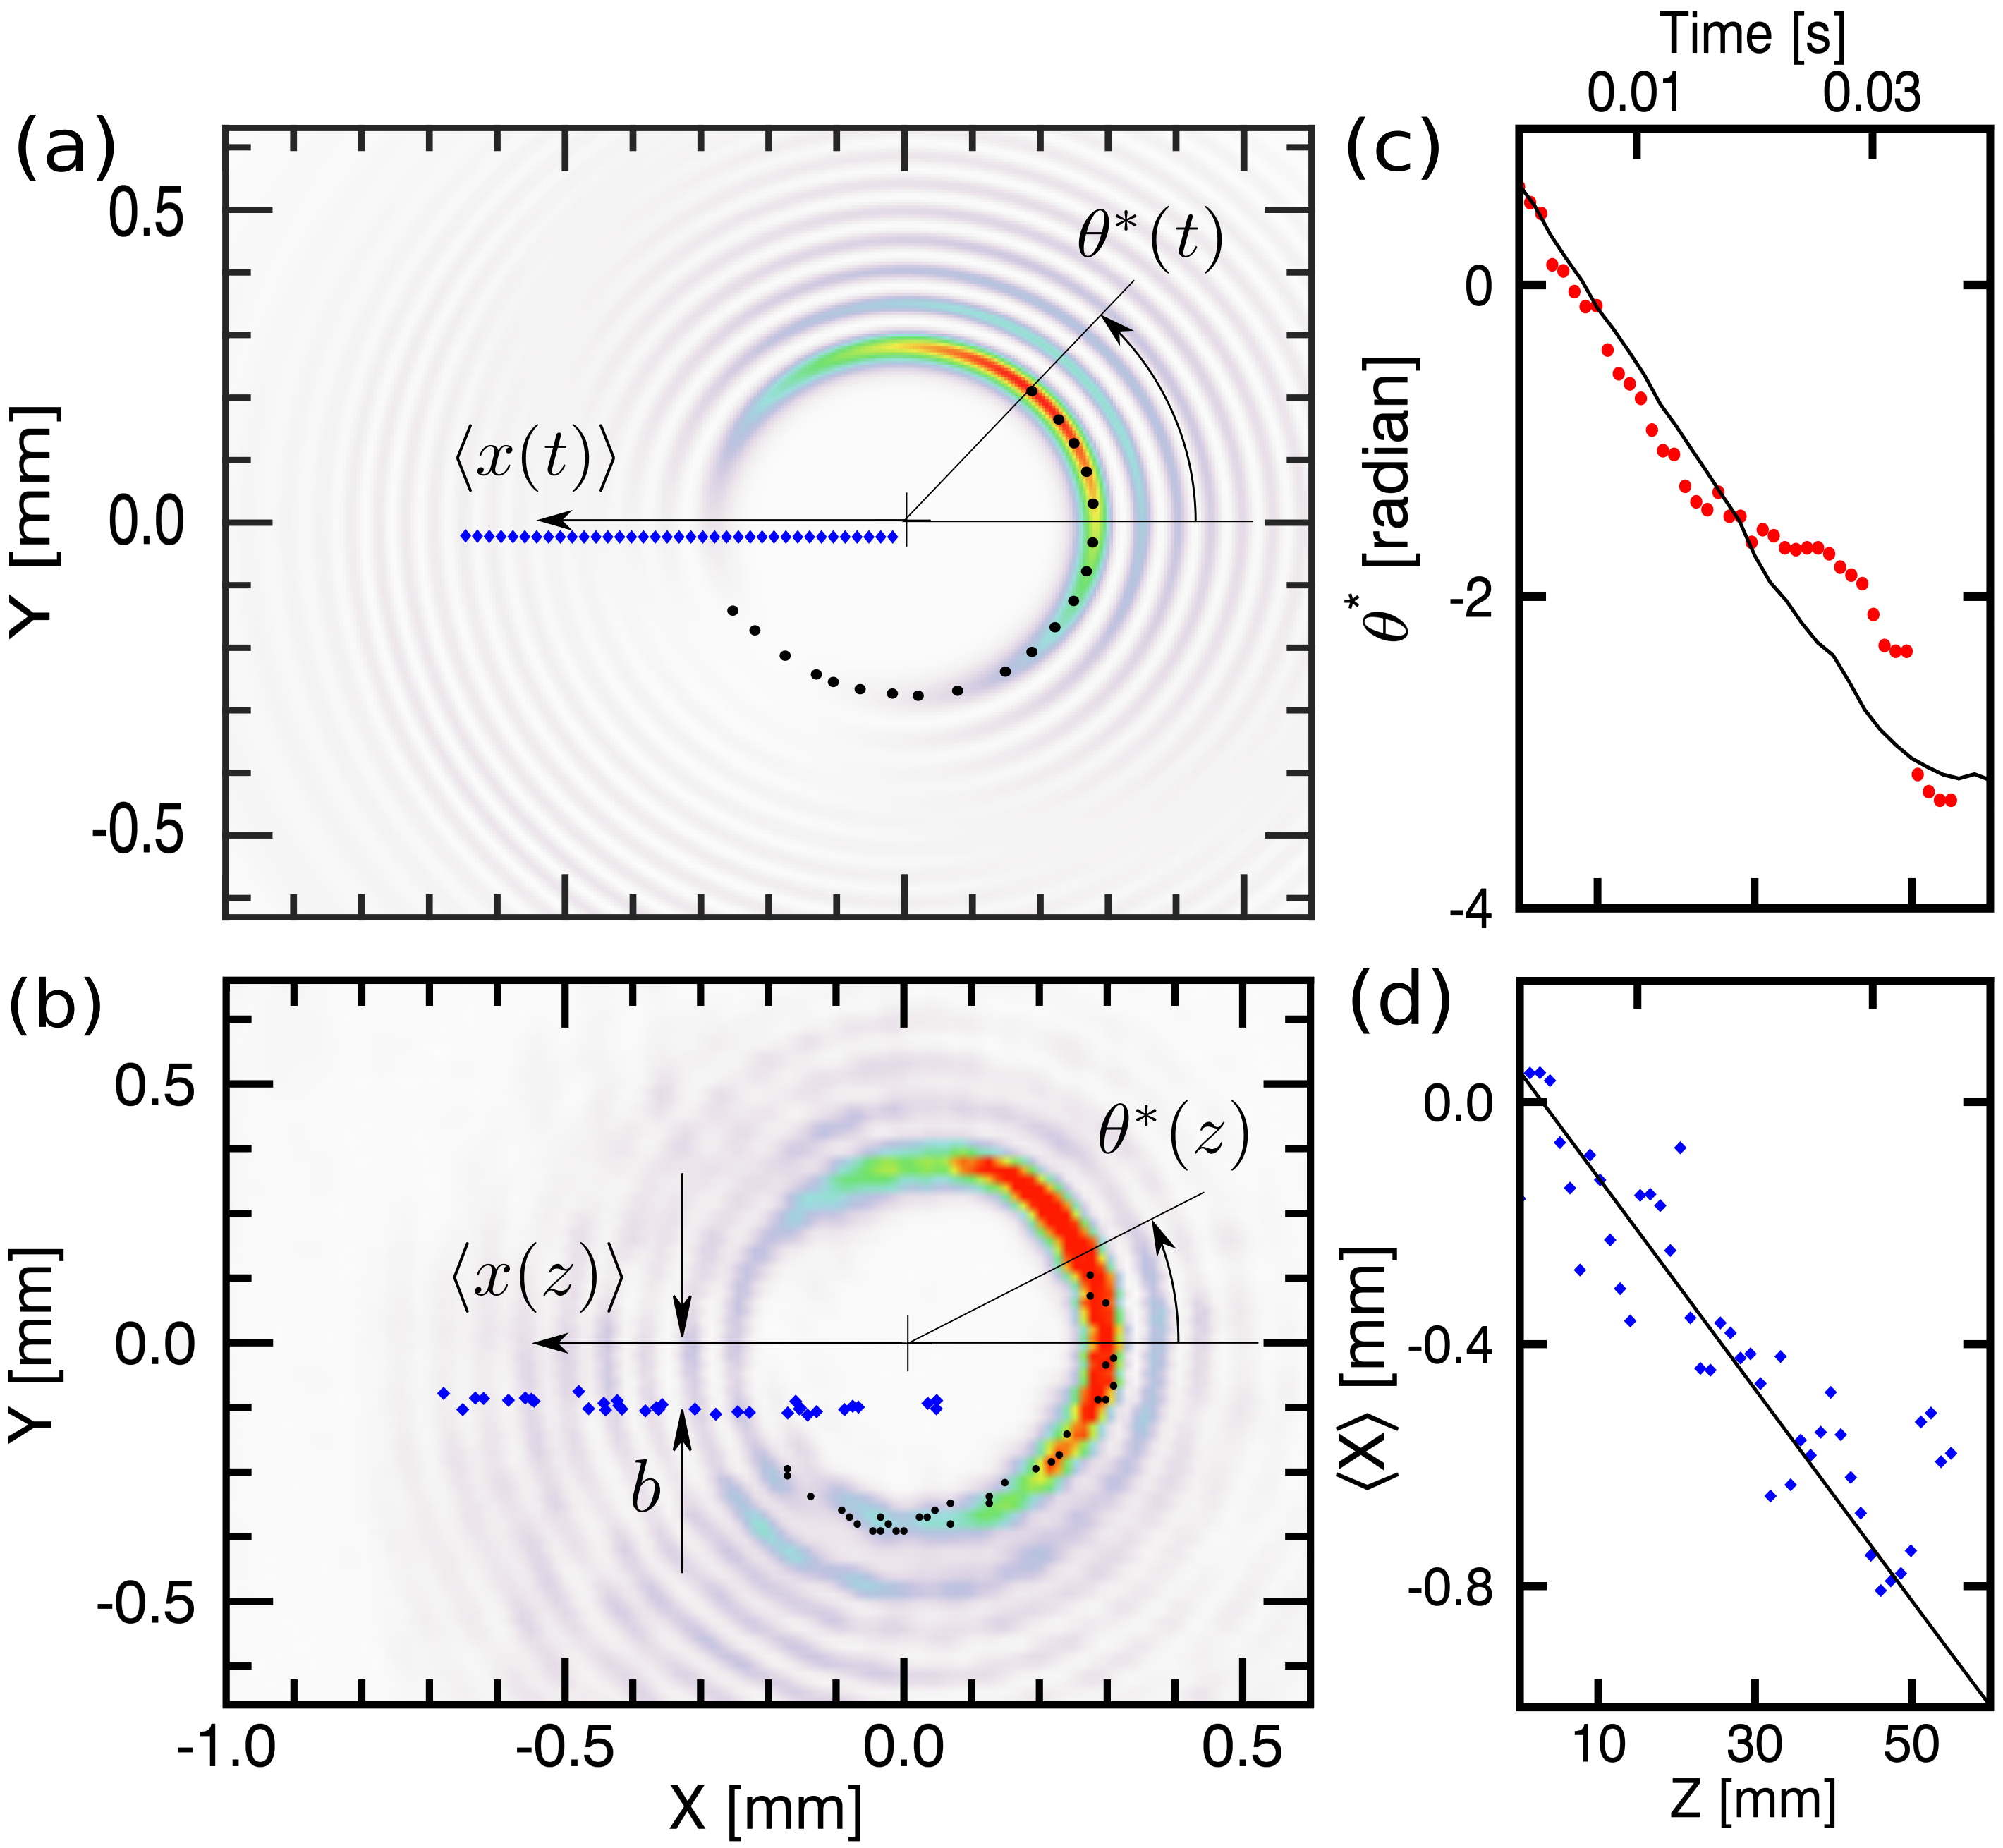
\includegraphics[width=\columnwidth]{translation05}
  \caption{Translation of a rotating wave packet.
  (a) Simulation of an accelerating state with $n = 20$, 
  $\nu = 16$ and $\nu' = 17$.  The image shows a region of interest
  around the center of
  the probability density $\rho(\vec{r},t)$.  Discrete points show
  the time evolution of the the most probable 
  position $\vec{r}^\ast(t)$, which circulates, 
  and of the expectation value
  of the position $\braket{\vec{r}(t)}$, which translates.
  (b) Corresponding experimental realization.
  (c) Time evolution of the mode position $\theta^\ast(t)$
  in the simulation (solid curve) compared with 
  $\theta^\ast(z)$ from the experimental data (discrete points).
  (d) Time evolution of the simulated wave packet's mean position
  $\braket{x(t)}$ compared with the position of the experimental
  center of brightness, $\braket{x(z)}$.
  }
  \label{fig:translation}
\end{figure}

Although the confined particle's classical acceleration
can be accounted for by the influence
of boundary conditions,
its rate of circulation is less straightforward to interpret.
The classical angular momentum carried by an
accelerating solenoidal wave packet is
\begin{subequations}
  \label{eq:Lz}
  \begin{align}
    \label{eq:solenoidLz}
    L_z^{(c)}
    & = m \alpha^2 R^2 \Omega \\
    & =
      2 \frac{j_{n+1,\nu'}^2 j_{n,\nu}^2}{
      (j_{n + 1,\nu'}^2 - j_{n,\nu}^2)^3} \, \hbar ,
  \end{align}
\end{subequations}
which differs from the state's quantum mechanical angular momentum,
\begin{equation}
  \label{eq:solenoidQLz}
  \braket{L_z} = \left(n + \frac{1}{2} \right) \hbar.
\end{equation}
Indeed, $L_z^{(c)}$ and $\braket{L_z}$ can have opposite signs
depending on the choice of radial quantum numbers $\nu$ and $\nu'$.
The solenoidal states represented in Figs.~\ref{fig:light}(a) 
and \ref{fig:light}(b), for example, 
have opposite classical angular
momentum even though they carry the same quantum mechanical
angular momentum.
Unconfined solenoidal states also carry classical angular
momentum
\begin{equation}
L_z^{(c)} 
=
m 
\left[\braket{\vec{r}(0)} \times \frac{d \braket{\vec{r}(t)}}{dt}\right]
\cdot \hat{z}
\end{equation}
that is equal to the confined value from
Eq.~\eqref{eq:Lz}
and generally differs from the quantum-mechanical
value, Eq.~\eqref{eq:solenoidQLz}.
Similar discrepancies between classical and quantum mechanical
angular momenta have been been observed in the spatial structure
of holographically-patterned electron
beams \cite{schattschneider14}.
A comprehensive paradigm for understanding these discrepancies and their physical consequences remains elusive.


\section{Acknowledgment}
This work was supported primarily
by the National Science Foundation under award number
DMR-1305875 and in part by the MRSEC program
of the NSF through award number
DMR-1420073.
The authors are grateful for helpful conversations
with David Pine, Paul Chaikin and
Aaron Yevick.

